\subsubsection{Invasion Percolation}

%which maps
%exactly into the Prim's method for minimal spanning tree problem \cite{prim1957shortest,barabasi1996invasion}.
%We first review Invasion Percolation, which  simulates the distribution of fluid
Invasion Percolation \cite{wilkinson1983invasion} simulates the distribution of fluid slowly %replacing/
invading porous media, e.g., water replacing the air in a porous rock.
We focus on a variant called bond IP (BIP), where ``bonds'' indicate edges in a lattice, and present the graph-based description by \citeauthor{barabasi1996invasion} (\citeyear{barabasi1996invasion}).
Given initial node(s) and a graph whose edges are assigned independent random values,
% Each node has a flag indicating whether Initial nodes are 
BIP iteratively marks the nodes.
Once assigned, the random value on each edge never changes.  The initial nodes are marked by default.
In each iteration marks an unmarked node to which the least-value outgoing edge leads.
Marked nodes represent the porous sites whose air is replaced by the water (invader).
% The algorithm proceeds as follows:
\citeauthor{barabasi1996invasion} (\citeyear{barabasi1996invasion}) showed that
this algorithm is equivalent to applying Prim's method for MST \cite{prim1957shortest} on a randomly weighted graph:
Prim's method constructs an MST by iteratively adding a neighboring edge with the least edge costs
to the existing tree.
% Since Prim's method works on any undirected graph, we can run BIP on arbitrary dimensions and graphs.
% Since Prim's method finds a MST minimizing the edge cost sum, BIP simulates the water greedily trying to expand with the least friction pathways.

% \begin{itemize}
%  \item Mark all initial nodes. 
%  \item In each iteration, select an edge with the least value among the edges which starts from marked nodes, then mark the destination of the edge.
% \end{itemize}

\begin{figure}[tb]
 \centering
 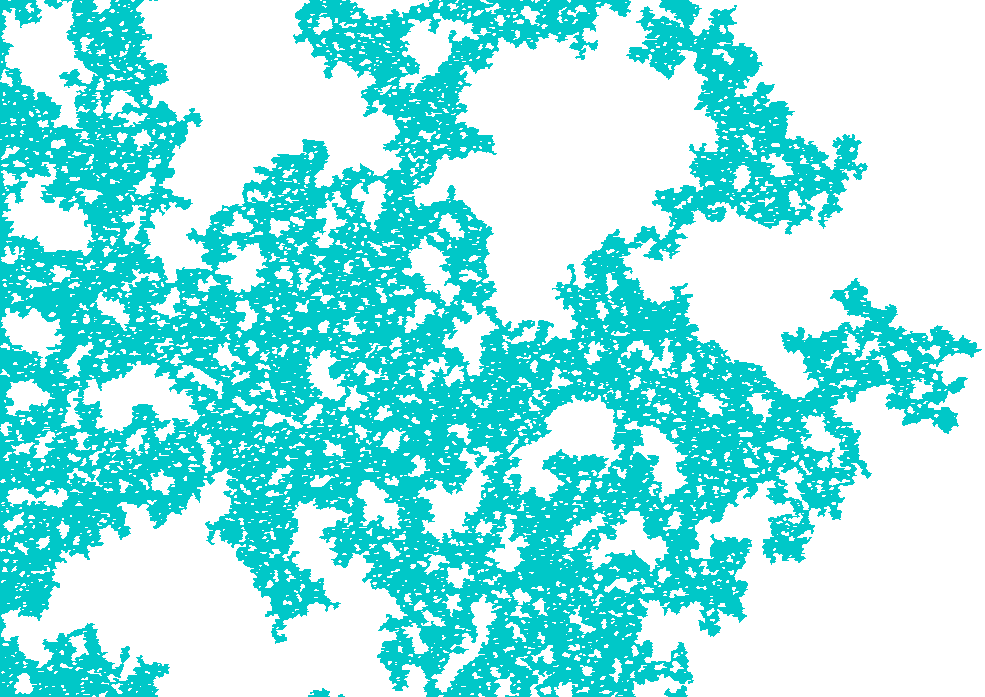
\includegraphics[width=0.4\linewidth]{img/static/ip.png}
 \caption{Invasion Percolation on 2-dimensional lattice}
 \label{fig:ip}
\end{figure}

\refig{fig:ip} illustrates a 2-D lattice after running BIP for a while. The initial nodes are 
at the leftmost edge of the rectangular region, i.e. the fluid percolates from the left. The
resulting structure has holes of various sizes that the fluid has not invaded, due to
the high-valued edges surrounding the neighbors of the holes, which serve as an embankment preventing the water from invading. Since the random value
on each edge is fixed, the algorithm does not mark the nodes inside the hole until it marks all nodes with smaller
random values in the entire space outside the embankments.
This behavior is critical to forming a fractal structure.

